\chapter{Introduction}
\label{chapter:introduction}

\setlength{\epigraphwidth}{0.43\textwidth}
\epigraph{
Out of S. Okubo's effect\\
At high temperature\\
A fur coat is sewed for the Universe\\
Shaped for its crooked figure
}{A. D. Sakharov \cite{Sakharov1991}}

We interact with matter every day. Even you, the reader, are probably made out of matter! However, antimatter is so rare that it is considered to cost a few hundred millions Swiss francs per gram \cite{DeRujula2001}, making it the most expensive substance in the universe. Why does such a stunning difference in the abundance exist?

First step to solving this problem is to define what are the required conditions that would allow the disbalance to evolve. Those conditions \cite{Dubbers2011} were described \cite{Sakharov1991} by Andrei Sakharov in 1967:

\begin{itemize}
	\item Violation of baryon number conservation
	\item \textit{C}- and \textit{CP}-symmetry violation
	\item Processes take place far from thermal equilibrium
\end{itemize}

Let's take a look at the \textit{CP}-symmetry and prove that a non-zero electric dipole moment of an elementary particle would indeed break it. We would select neutron as a particle of choice.

The neutron in the ground state has spin of $I = 1/2$ and can be characterised completely by a single quantum number of a spin projection $m_I = \pm 1/2$. We can write down a Hamiltonian \cite{Golub1994} of this neutron in external electric and magnetic fields $\vec{E}$ and $\vec{B}$:

\begin{equation}
	\mathcal{H} = -\frac{d_n \vec{I} \cdot \vec{E} + \mu_n \vec{I} \cdot \vec{B}}{I}
	\label{eq:neutron_hamiltonian}
\end{equation}

with $d_n$ and $\mu_n$ being the electric and magnetic moments of the neutron \cite{Golub1972}.

It does not make sense to discuss the potential violation of the symmetries before we define them.  Fundamental symmetries are blended into the fabric of our Universe by providing sufficient conditions \cite{Noether1918} for the conservation laws. In our analysis we would consider three symmetries of the Standard Model: \textit{C}, \textit{P} and \textit{T}.

\begin{itemize}
	\item (C)harge –-- replaces every particle with its antiparticle: $q \rightarrow -q$
	\item (P)arity --- inverts the physical space: $\vec{r} \rightarrow -\vec{r}$
	\item (T)ime --- turns the time back: $t \rightarrow -t$
\end{itemize}

How would the \textit{P} and \textit{T} inversions affect \cite{Dubbers2011} the Hamiltonian from Eq. \ref{eq:neutron_hamiltonian}?

Parity transformation only act on a polar vector of the electric field: $\vec{E} \rightarrow -\vec{E}$, both $\vec{B}$ and $\vec{I}$ are conserved. This brings us to
\begin{equation}
	\textit{P}\mathcal{H} = -\frac{d_n \vec{I} \cdot \left(-\vec{E}\right) + \mu_n \vec{I} \cdot \vec{B}}{I} \neq \mathcal{H}
	\label{eq:neutron_hamiltonian_P}
\end{equation}

Time reversal would affect only axial vectors $\vec{B}$ and $\vec{I}$: $\vec{B} \rightarrow -\vec{B},\ \vec{I} \rightarrow -\vec{I}$, the field $\vec{E}$ is left as is:
\begin{equation}
	\textit{T}\mathcal{H} = -\frac{d_n \left(-\vec{I}\right) \cdot \vec{E} + \mu_n \left(-\vec{I}\right) \cdot \left( -\vec{B} \right)}{I} \neq \mathcal{H}
	\label{eq:neutron_hamiltonian_T}
\end{equation}

Assuming that the \textit{CPT} invariance \cite{Schwinger1951} is conserved, we derive the violation of a \textit{CP}-symmetry, which provides us motivation to measure the EDM of the neutron.

\textit{"Wait a minute,"} could have said an attentive reader at this point. "Does not Standard Model predict a non-zero EDM of the neutron already? I am still not convinced why would you want to conduct this experiment."

And an attentive reader would have had a completely fair point! Indeed, Standard Model predicts \cite{Khriplovich1982} the following:
\begin{equation}
	d_n \approx 2 \cdot 10^{-32}\ e \cdot \text{cm}
\end{equation}

However, we would still like to measure $d_n$ for the reasons listed below:
\begin{itemize}
	\item The only way to prove the theory is to check it experimentally. So far no one has measured $d_n$ with a precision close to the predicted value
	\item The result that can be achieved by using Standard Model is too weak to explain the baryogenesis \cite{Dubbers2011}, yet baryogenesis has clearly happened
	\item If we go beyond Standard Model to find a mechanism, through which the Universe as we know it could have been formed, we need to cut off theories that do not agree with experimental data. This is something that this experiment does perfectly: on the Fig. \ref{fig:edm_history} one can see all theoretical models that the measurement of the neutron EDM has ruled out, allowing the scientists to focus on more prominent theories.
\end{itemize}

\begin{figure}[h]
	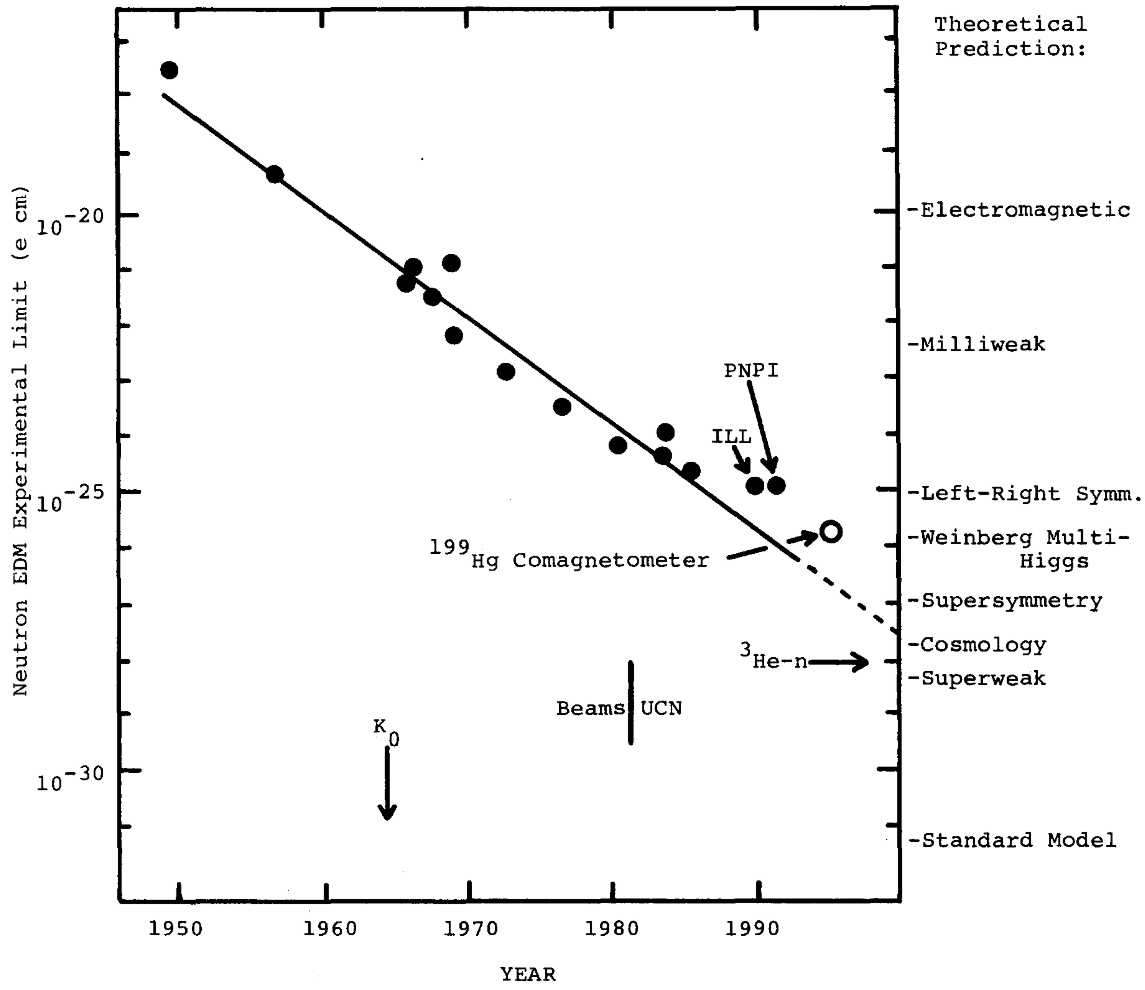
\includegraphics[width=\textwidth]{img/history_of_nedm_measurements}
	\caption{Measurement history of the neutron EDM \cite{Golub1994}}
	\label{fig:edm_history}
\end{figure}

Hopefully these reasons would convince even the most demanding reader in the need to conduct the n2EDM experiment. But what is \textit{n2EDM} exactly? We will try to explain that in the next chapter.
